\documentclass[11pt]{article}
\usepackage[textwidth=18.0cm, textheight=23.0cm, top=2.0cm]{geometry}
\usepackage{pst-all}
\usepackage{amssymb}
\usepackage{tikz}
\usepackage{underscore}\begin{document}
\pagestyle{empty}


ClassName: \underline{\textbf{Class_02.2bp-48}}
\par
BinSize: \underline{\textbf{30 × 30}}
\par
ReduceSize: \underline{\textbf{30 × 30}}
\par
TypeNum: \underline{\textbf{67}}
\par
Num: \underline{\textbf{100}}
\par
OutS: \underline{\textbf{3600}}
\par
InS: \underline{\textbf{2986}}
\par
Rate: \underline{\textbf{0.829}}
\par
UB: \underline{\textbf{4}}
\par
LB0: \underline{\textbf{4}}
\par
LB: \underline{\textbf{4}}
\par
LBWithCut: \underline{\textbf{4}}
\par
NodeCut: \underline{\textbf{0}}
\par
ExtendedNodeCnt: \underline{\textbf{1}}
\par
GenNodeCnt: \underline{\textbf{1}}
\par
PrimalNode: \underline{\textbf{0}}
\par
ColumnCount: \underline{\textbf{4}}
\par
TotalCutCount: \underline{\textbf{0}}
\par
RootCutCount: \underline{\textbf{0}}
\par
LPSolverCnt: \underline{\textbf{1}}
\par
PricingSolverCnt: \underline{\textbf{0}}
\par
BranchAndBoundNum: \underline{\textbf{1}}
\par
isOpt: \underline{\textbf{true}}
\par
TimeOnInitSolution: \underline{\textbf{0.000 s}}
\par
TimeOnPrimal: \underline{\textbf{0.000 s}}
\par
TimeOnPricing: \underline{\textbf{0.000 s}}
\par
TimeOnRmp: \underline{\textbf{0.078 s}}
\par
TotalTime: \underline{\textbf{0.141 s}}
\par
\newpage


\begin{tikzpicture}[shorten >=1pt,scale=1.0,every node/.style={scale=1.0},->]
\tikzstyle{vertex}=[circle,fill=black!25,minimum size=14pt,inner sep=0pt]
\filldraw[fill=gray!40!white, draw=black] (0,0) rectangle (15.0,15.0);
\foreach \name/\x/\y/\w/\h in {10x10/0.0/0.0/5.0/5.0,10x10/5.0/0.0/5.0/5.0,10x9/10.0/0.0/5.0/4.5,10x9/0.0/5.0/5.0/4.5,9x10/9.0/10.0/4.5/5.0,9x10/0.0/9.5/4.5/5.0,9x9/5.0/5.0/4.5/4.5,8x10/4.5/9.5/4.0/5.0,7x9/9.5/5.0/3.5/4.5,4x10/13.0/5.0/2.0/5.0,3x10/13.5/10.0/1.5/5.0,10x1/10.0/4.5/5.0/0.5,8x1/9.0/9.5/4.0/0.5,8x1/4.5/14.5/4.0/0.5,8x1/0.5/14.5/4.0/0.5,1x6/8.5/9.5/0.5/3.0,1x5/8.5/12.5/0.5/2.5,1x1/0.0/14.5/0.5/0.5}
\filldraw[fill=white!40!white, draw=black] (\x,\y) rectangle node[draw] (\name) {\name} ++(\w,\h);
\end{tikzpicture}


w =10 , h =10 , x =0 , y =0 , v =100
\par
w =10 , h =10 , x =10 , y =0 , v =100
\par
w =10 , h =9 , x =20 , y =0 , v =90
\par
w =10 , h =9 , x =0 , y =10 , v =90
\par
w =9 , h =10 , x =18 , y =20 , v =90
\par
w =9 , h =10 , x =0 , y =19 , v =90
\par
w =9 , h =9 , x =10 , y =10 , v =81
\par
w =8 , h =10 , x =9 , y =19 , v =80
\par
w =7 , h =9 , x =19 , y =10 , v =63
\par
w =4 , h =10 , x =26 , y =10 , v =40
\par
w =3 , h =10 , x =27 , y =20 , v =30
\par
w =10 , h =1 , x =20 , y =9 , v =10
\par
w =8 , h =1 , x =18 , y =19 , v =8
\par
w =8 , h =1 , x =9 , y =29 , v =8
\par
w =8 , h =1 , x =1 , y =29 , v =8
\par
w =1 , h =6 , x =17 , y =19 , v =6
\par
w =1 , h =5 , x =17 , y =25 , v =5
\par
w =1 , h =1 , x =0 , y =29 , v =1
\par
\newpage


\begin{tikzpicture}[shorten >=1pt,scale=1.0,every node/.style={scale=1.0},->]
\tikzstyle{vertex}=[circle,fill=black!25,minimum size=14pt,inner sep=0pt]
\filldraw[fill=gray!40!white, draw=black] (0,0) rectangle (15.0,15.0);
\foreach \name/\x/\y/\w/\h in {10x8/0.0/0.0/5.0/4.0,9x8/5.0/0.0/4.5/4.0,10x7/7.5/9.0/5.0/3.5,7x10/8.5/4.0/3.5/5.0,5x2/0.5/9.0/2.5/1.0,6x9/12.0/0.0/3.0/4.5,6x9/12.0/4.5/3.0/4.5,10x5/7.5/12.5/5.0/2.5,5x10/6.0/4.0/2.5/5.0,5x10/3.5/4.0/2.5/5.0,5x10/0.0/10.0/2.5/5.0,5x9/12.5/9.0/2.5/4.5,8x5/3.5/10.0/4.0/2.5,8x5/3.5/12.5/4.0/2.5,5x8/9.5/0.0/2.5/4.0,7x4/0.0/4.0/3.5/2.0,2x10/2.5/10.0/1.0/5.0,9x2/3.0/9.0/4.5/1.0,5x3/12.5/13.5/2.5/1.5,7x2/0.0/6.0/3.5/1.0,7x2/0.0/7.0/3.5/1.0,7x1/0.0/8.0/3.5/0.5,6x1/0.5/8.5/3.0/0.5,1x3/0.0/8.5/0.5/1.5}
\filldraw[fill=white!40!white, draw=black] (\x,\y) rectangle node[draw] (\name) {\name} ++(\w,\h);
\end{tikzpicture}


w =10 , h =8 , x =0 , y =0 , v =80
\par
w =9 , h =8 , x =10 , y =0 , v =72
\par
w =10 , h =7 , x =15 , y =18 , v =70
\par
w =7 , h =10 , x =17 , y =8 , v =70
\par
w =5 , h =2 , x =1 , y =18 , v =10
\par
w =6 , h =9 , x =24 , y =0 , v =54
\par
w =6 , h =9 , x =24 , y =9 , v =54
\par
w =10 , h =5 , x =15 , y =25 , v =50
\par
w =5 , h =10 , x =12 , y =8 , v =50
\par
w =5 , h =10 , x =7 , y =8 , v =50
\par
w =5 , h =10 , x =0 , y =20 , v =50
\par
w =5 , h =9 , x =25 , y =18 , v =45
\par
w =8 , h =5 , x =7 , y =20 , v =40
\par
w =8 , h =5 , x =7 , y =25 , v =40
\par
w =5 , h =8 , x =19 , y =0 , v =40
\par
w =7 , h =4 , x =0 , y =8 , v =28
\par
w =2 , h =10 , x =5 , y =20 , v =20
\par
w =9 , h =2 , x =6 , y =18 , v =18
\par
w =5 , h =3 , x =25 , y =27 , v =15
\par
w =7 , h =2 , x =0 , y =12 , v =14
\par
w =7 , h =2 , x =0 , y =14 , v =14
\par
w =7 , h =1 , x =0 , y =16 , v =7
\par
w =6 , h =1 , x =1 , y =17 , v =6
\par
w =1 , h =3 , x =0 , y =17 , v =3
\par
\newpage


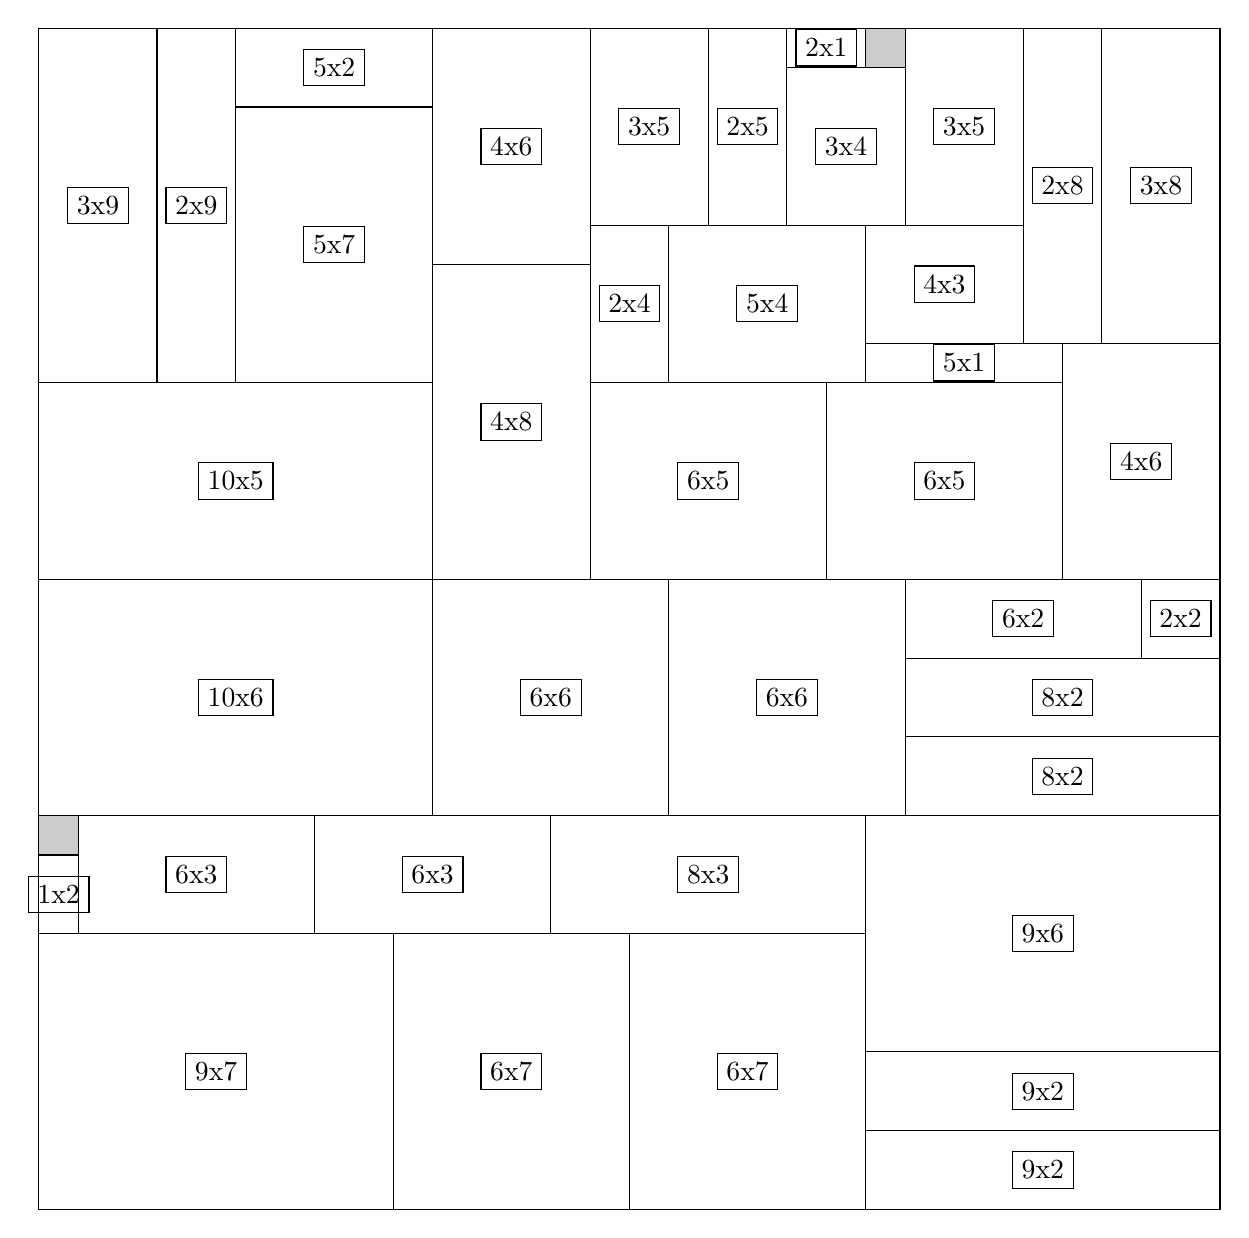
\begin{tikzpicture}[shorten >=1pt,scale=1.0,every node/.style={scale=1.0},->]
\tikzstyle{vertex}=[circle,fill=black!25,minimum size=14pt,inner sep=0pt]
\filldraw[fill=gray!40!white, draw=black] (0,0) rectangle (15.0,15.0);
\foreach \name/\x/\y/\w/\h in {9x7/0.0/0.0/4.5/3.5,10x6/0.0/5.0/5.0/3.0,10x5/0.0/8.0/5.0/2.5,6x7/4.5/0.0/3.0/3.5,6x7/7.5/0.0/3.0/3.5,6x6/5.0/5.0/3.0/3.0,6x6/8.0/5.0/3.0/3.0,5x7/2.5/10.5/2.5/3.5,4x8/5.0/8.0/2.0/4.0,6x5/7.0/8.0/3.0/2.5,6x5/10.0/8.0/3.0/2.5,3x9/0.0/10.5/1.5/4.5,8x3/6.5/3.5/4.0/1.5,4x6/5.0/12.0/2.0/3.0,4x6/13.0/8.0/2.0/3.0,3x8/13.5/11.0/1.5/4.0,5x4/8.0/10.5/2.5/2.0,9x2/10.5/0.0/4.5/1.0,9x2/10.5/1.0/4.5/1.0,6x3/3.5/3.5/3.0/1.5,6x3/0.5/3.5/3.0/1.5,2x9/1.5/10.5/1.0/4.5,8x2/11.0/5.0/4.0/1.0,8x2/11.0/6.0/4.0/1.0,2x8/12.5/11.0/1.0/4.0,3x5/11.0/12.5/1.5/2.5,3x5/7.0/12.5/1.5/2.5,6x2/11.0/7.0/3.0/1.0,4x3/10.5/11.0/2.0/1.5,3x4/9.5/12.5/1.5/2.0,5x2/2.5/14.0/2.5/1.0,9x6/10.5/2.0/4.5/3.0,2x5/8.5/12.5/1.0/2.5,2x4/7.0/10.5/1.0/2.0,5x1/10.5/10.5/2.5/0.5,2x2/14.0/7.0/1.0/1.0,2x1/9.5/14.5/1.0/0.5,1x2/0.0/3.5/0.5/1.0}
\filldraw[fill=white!40!white, draw=black] (\x,\y) rectangle node[draw] (\name) {\name} ++(\w,\h);
\end{tikzpicture}


w =9 , h =7 , x =0 , y =0 , v =63
\par
w =10 , h =6 , x =0 , y =10 , v =60
\par
w =10 , h =5 , x =0 , y =16 , v =50
\par
w =6 , h =7 , x =9 , y =0 , v =42
\par
w =6 , h =7 , x =15 , y =0 , v =42
\par
w =6 , h =6 , x =10 , y =10 , v =36
\par
w =6 , h =6 , x =16 , y =10 , v =36
\par
w =5 , h =7 , x =5 , y =21 , v =35
\par
w =4 , h =8 , x =10 , y =16 , v =32
\par
w =6 , h =5 , x =14 , y =16 , v =30
\par
w =6 , h =5 , x =20 , y =16 , v =30
\par
w =3 , h =9 , x =0 , y =21 , v =27
\par
w =8 , h =3 , x =13 , y =7 , v =24
\par
w =4 , h =6 , x =10 , y =24 , v =24
\par
w =4 , h =6 , x =26 , y =16 , v =24
\par
w =3 , h =8 , x =27 , y =22 , v =24
\par
w =5 , h =4 , x =16 , y =21 , v =20
\par
w =9 , h =2 , x =21 , y =0 , v =18
\par
w =9 , h =2 , x =21 , y =2 , v =18
\par
w =6 , h =3 , x =7 , y =7 , v =18
\par
w =6 , h =3 , x =1 , y =7 , v =18
\par
w =2 , h =9 , x =3 , y =21 , v =18
\par
w =8 , h =2 , x =22 , y =10 , v =16
\par
w =8 , h =2 , x =22 , y =12 , v =16
\par
w =2 , h =8 , x =25 , y =22 , v =16
\par
w =3 , h =5 , x =22 , y =25 , v =15
\par
w =3 , h =5 , x =14 , y =25 , v =15
\par
w =6 , h =2 , x =22 , y =14 , v =12
\par
w =4 , h =3 , x =21 , y =22 , v =12
\par
w =3 , h =4 , x =19 , y =25 , v =12
\par
w =5 , h =2 , x =5 , y =28 , v =10
\par
w =9 , h =6 , x =21 , y =4 , v =54
\par
w =2 , h =5 , x =17 , y =25 , v =10
\par
w =2 , h =4 , x =14 , y =21 , v =8
\par
w =5 , h =1 , x =21 , y =21 , v =5
\par
w =2 , h =2 , x =28 , y =14 , v =4
\par
w =2 , h =1 , x =19 , y =29 , v =2
\par
w =1 , h =2 , x =0 , y =7 , v =2
\par
\newpage


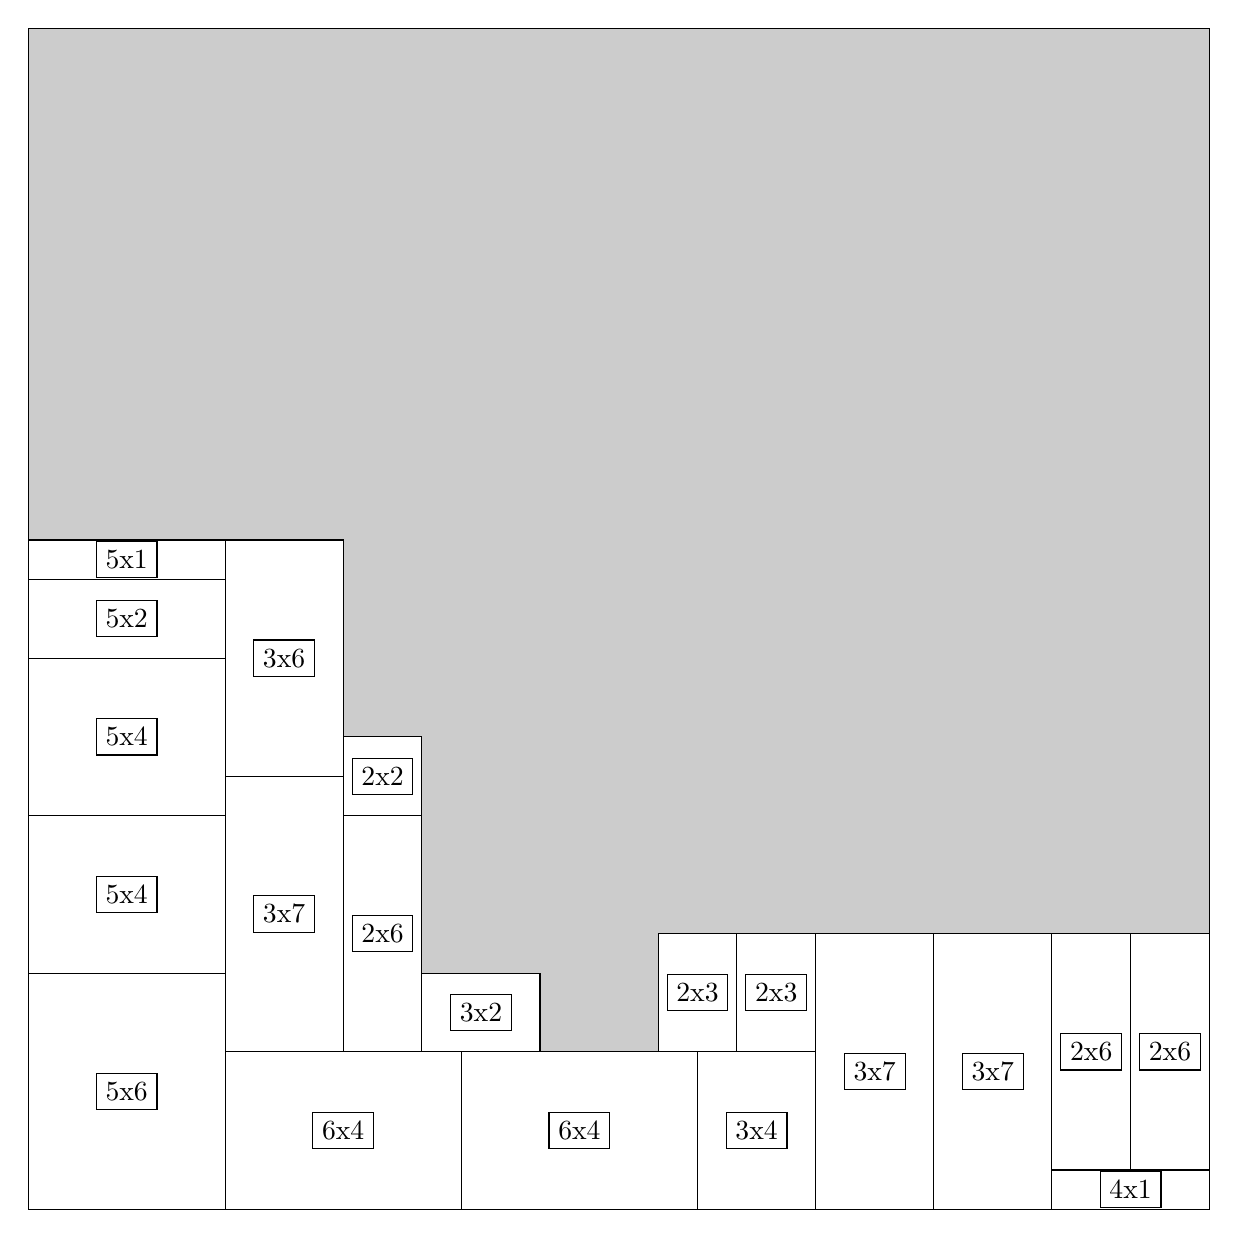
\begin{tikzpicture}[shorten >=1pt,scale=1.0,every node/.style={scale=1.0},->]
\tikzstyle{vertex}=[circle,fill=black!25,minimum size=14pt,inner sep=0pt]
\filldraw[fill=gray!40!white, draw=black] (0,0) rectangle (15.0,15.0);
\foreach \name/\x/\y/\w/\h in {5x6/0.0/0.0/2.5/3.0,6x4/2.5/0.0/3.0/2.0,6x4/5.5/0.0/3.0/2.0,3x7/10.0/0.0/1.5/3.5,3x7/11.5/0.0/1.5/3.5,3x7/2.5/2.0/1.5/3.5,5x4/0.0/3.0/2.5/2.0,5x4/0.0/5.0/2.5/2.0,3x6/2.5/5.5/1.5/3.0,3x4/8.5/0.0/1.5/2.0,2x6/13.0/0.5/1.0/3.0,2x6/14.0/0.5/1.0/3.0,2x6/4.0/2.0/1.0/3.0,5x2/0.0/7.0/2.5/1.0,3x2/5.0/2.0/1.5/1.0,2x3/9.0/2.0/1.0/1.5,2x3/8.0/2.0/1.0/1.5,5x1/0.0/8.0/2.5/0.5,4x1/13.0/0.0/2.0/0.5,2x2/4.0/5.0/1.0/1.0}
\filldraw[fill=white!40!white, draw=black] (\x,\y) rectangle node[draw] (\name) {\name} ++(\w,\h);
\end{tikzpicture}


w =5 , h =6 , x =0 , y =0 , v =30
\par
w =6 , h =4 , x =5 , y =0 , v =24
\par
w =6 , h =4 , x =11 , y =0 , v =24
\par
w =3 , h =7 , x =20 , y =0 , v =21
\par
w =3 , h =7 , x =23 , y =0 , v =21
\par
w =3 , h =7 , x =5 , y =4 , v =21
\par
w =5 , h =4 , x =0 , y =6 , v =20
\par
w =5 , h =4 , x =0 , y =10 , v =20
\par
w =3 , h =6 , x =5 , y =11 , v =18
\par
w =3 , h =4 , x =17 , y =0 , v =12
\par
w =2 , h =6 , x =26 , y =1 , v =12
\par
w =2 , h =6 , x =28 , y =1 , v =12
\par
w =2 , h =6 , x =8 , y =4 , v =12
\par
w =5 , h =2 , x =0 , y =14 , v =10
\par
w =3 , h =2 , x =10 , y =4 , v =6
\par
w =2 , h =3 , x =18 , y =4 , v =6
\par
w =2 , h =3 , x =16 , y =4 , v =6
\par
w =5 , h =1 , x =0 , y =16 , v =5
\par
w =4 , h =1 , x =26 , y =0 , v =4
\par
w =2 , h =2 , x =8 , y =10 , v =4
\par
\newpage


\end{document}